\section{Introduction}

%\lrcomment{Intro is still a bit too long, we can probably cut down on the first
%4 paragraphs.}
%\abc{reduced some of the material}
\nancomment{1. docker and docker registry trend
	2. content addressable are using for 
	3. But:we download and ..found
	4. the need to provide a large scale analysis
	5. findings and suggests
	}
	
=======old version=====================

Recently, \emph{containers}~\cite{process-containers-linux} have
gained significant traction as an alternative to the virtual
machines~\cite{rosenblum2005virtual} for virtualization both on
premises and in the cloud---polls suggest that 87\% of enterprises are
at various stages of adopting containers, and they are expected to
constitute a lucrative \$2.5 billion
market~\cite{container-grow-by2020} by 2020.
%
In contrast to virtual machines, containers share the same kernel but
are isolated in terms of visibility (e.g., via
namespaces~\cite{man-namespaces}) and resources (e.g., via control
groups~\cite{kernel-doc-cgroups}). This enables containers to use
less memory and storage, start much faster, and typically incur less
execution overhead~\cite{Disco, felter2015updated,
	HypervisorsvsLightweight}.
	
A driving force for fast container
adoption is the popular Docker~\cite{docker} container management
framework. Docker combines process containerization with efficient and
effective packaging  of complete runtime environment
in so called {\em images}.
For efficiency, images are composed of independent,
shareable {\em layers} of files.
%
Both images
and layers are stored in a centralized \emph{registry} and accessed by clients as needed.
%
Docker Hub~\cite{docker-hub} is the most widely used registry, which currently
stores more than 500,000 public image repositories comprising of over 2 million layers.
The size of the registry 
is steadily increasing---we observed a linear growth of the
number of images in Docker Hub over a period from June to September 2017.


While the massive image dataset presents challenges to the registry
and client storage
infrastructure, storage for containers has remained a largely unexplored
area.
%
We believe one of the prime reasons is the limited understanding of what data
is stored inside containers.
%
This knowledge can help to improve the registry and container
storage infrastructure and ensure scalability of and fast accesses to the
registry service.
%
Existing work has focused on various aspects of
containerization~\cite{dockerssd, dockerfinder, analysisdockergithub,
slacker, dockervulnerabile}.
However, the registry and its contents have yet to be studied in detail.

In this paper, we perform the first, comprehensive, large-scale characterization
of the images and layers stored in the Docker Hub
registry~(\S\ref{sec:background}).
%
We download all latest publicly accessible images, which amount to 51~TB of
image data. Based on that dataset, we analyze traditional storage properties, such
as file count, data compression ratios, directory depths, as well as
Docker-specific properties, e.g., the number of layers per image, image popularity,
and the amount of layer sharing.

%\lrcomment{Would need to tie this in with Section 3, otherwise, we should remove
%this paragraph again?\nancomment{we can remove this paragraph}}

\begin{figure}
	\centering
	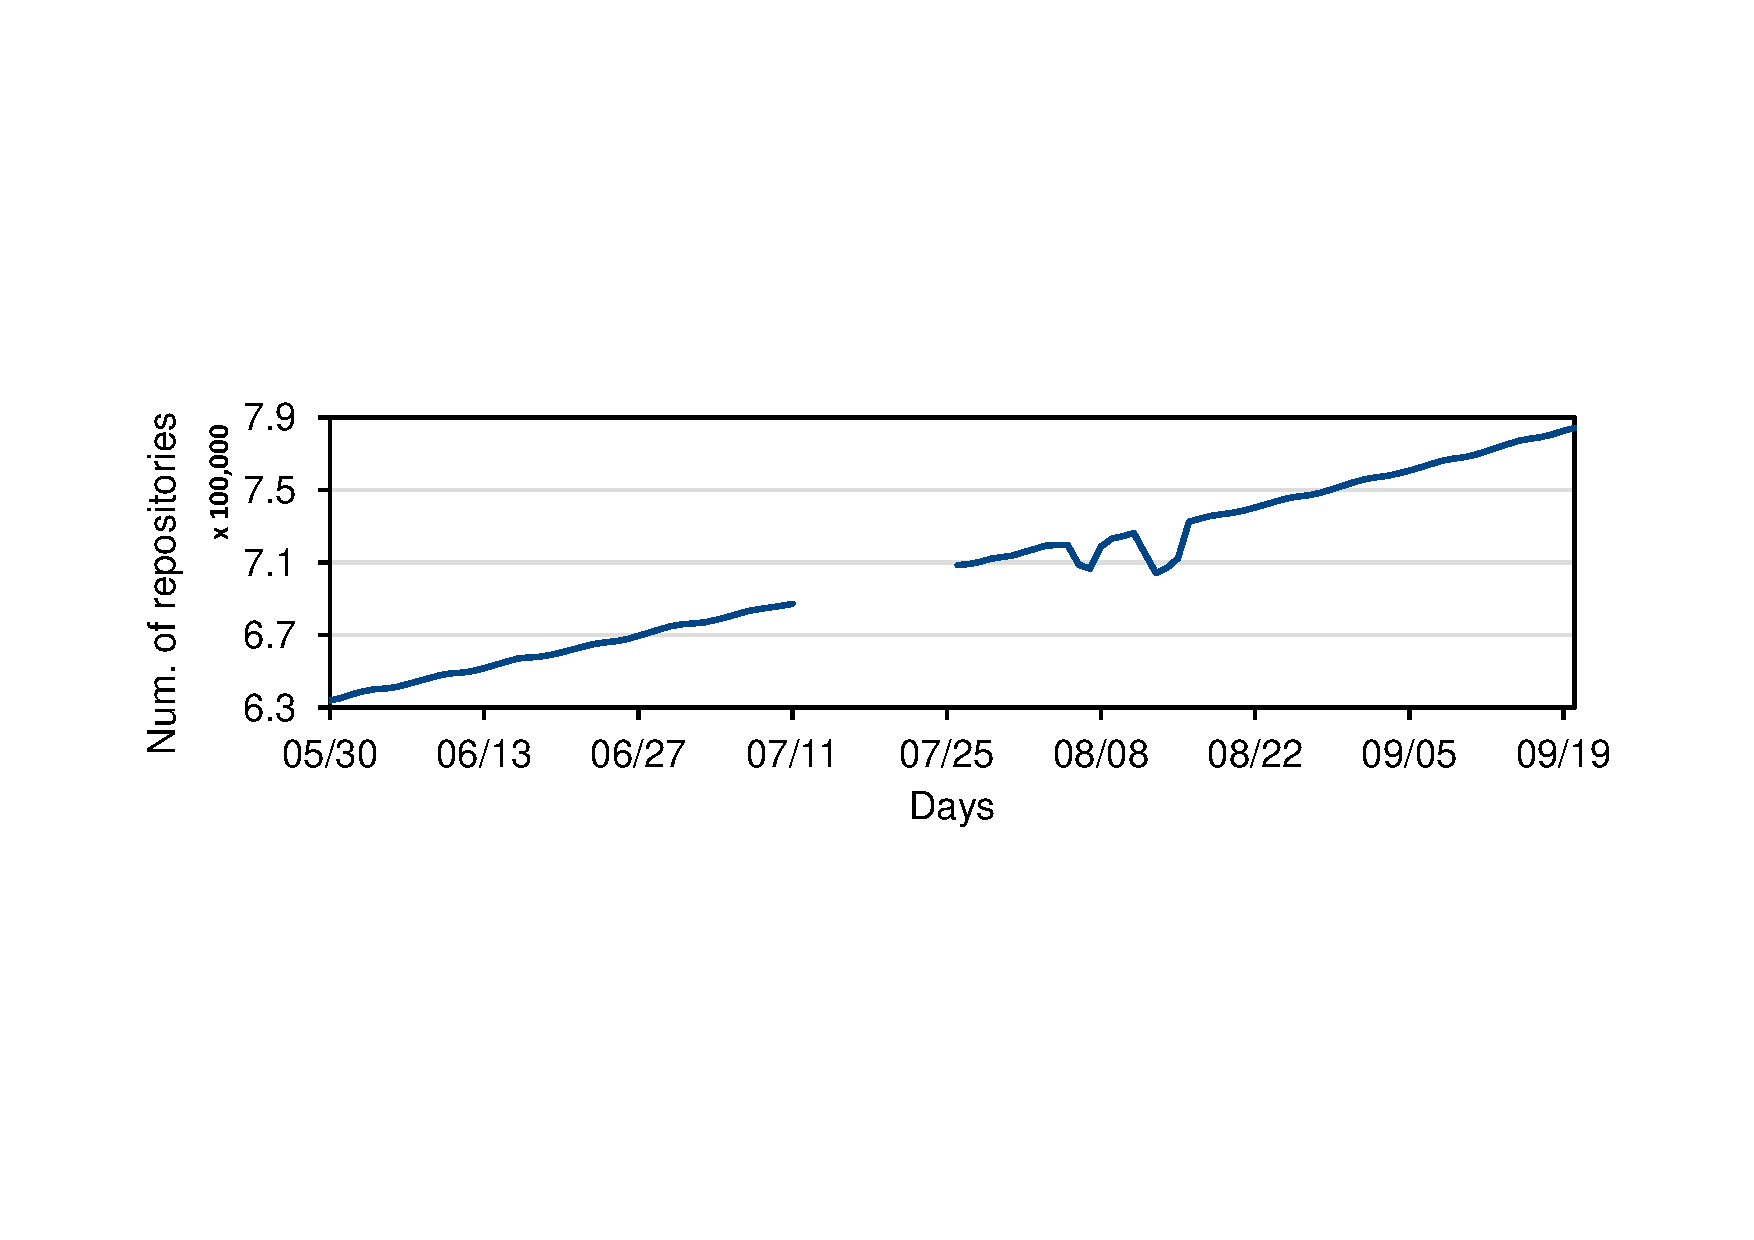
\includegraphics[width=0.5\textwidth]{graphs/image_growth.pdf}
	\caption{Total number of public repositories in Docker Hub
		from May 30 to September 20, 2017. Y axis starts
		at 630,000 repositories.
		%	   \vcomment{X axis label should be ``Date''.\nancomment{addressed all}}
		%	   \vcomment{Y axis label x100,000 ``is badly aligned''.}
		%	   \vcomment{Y axis label x100,000 ``is badly aligned''.}
	}
	\label{fig_image_growth}
\end{figure}

To download this large dataset, we overcome two
challenges~(\S\ref{sec:methodology}): i)~we provide an efficient way of identifying
all stored images as Docker Hub does not provide an API for this;
and ii)~we ensure the dataset is clean by handling
duplicates and removing links to broken or private images.
We plan to make all metadata (over 100GB of compressed
JSON files) publicly available.

Our analysis reveals several interesting insights~(\S\ref{sec:char}). 
We find that image
accesses are skewed towards a small number of popular images. Specifically,
90\% of repositories are pulled less than 300 times from the point of their
creation, while the largest number of pulls we record for an image is
over 600 million. This suggests that image caching is a viable improvement
for the registry.
%
The majority of layers are small in size and only show a low compression ratio.
50\% of the layers are smaller than 4 MB which holds both for compressed and 
uncompressed layers. This results in a median compression ratio of 2.6.
As compression is computationally intensive, storing small layers in the
registry uncompressed can improve latency during pulls as layers do not
have to be uncompressed locally anymore.

Our findings provide a first, quick insight in the Docker image dataset which
can help to improve the understanding of how Docker containers are structured.
%We discuss related work in~\S\ref{sec:related} and then conclude~(\S\ref{sec:conclusion}).

%This results in a compression ratio of \gap and shows the potential efffectiveness of
%compression\nancomment{add compression ratio}.
%\lrcomment{I thought layers are already compressed tarballs? How can we save space
%via compression?}\abc{ditto?}\nancomment{we can remove "save space"}
%Also, layers experience a large overlap of files with 10\% of all files
%appearing in more than 1 images. 
%This reveals potential for deduplication at
%file granularity \nancomment{docker already did this. we can remove this sentence}.

%   After discussing related work~(\S\ref{sec:related}),
%   the paper concludes~(\S\ref{sec:conclusion}).


%%%%%%%%%%%%%%%%%%%%%%%%%%%%%%%%%%%%%%%%%%%%%%%%%%%%%%%%%%%%%%%%%%%%%%%%%%%%%%
%                                                                            %
%                                OLD INTRO                                   %
%                                                                            %
%%%%%%%%%%%%%%%%%%%%%%%%%%%%%%%%%%%%%%%%%%%%%%%%%%%%%%%%%%%%%%%%%%%%%%%%%%%%%%

%For years, virtual machines served as a cornerstone of computing resource
%virtualization both on premises and in the cloud~\cite{rosenblum2005virtual}.
%%
%Recently, however, \emph{container-based} virtualization started to gain
%significant traction~\cite{process-containers-linux}.
%%
%According to polls, over 87\% of enterprises are at various stages of adopting
%containers; analysts also predict that by 2020, containers will constitute a
%lucrative \$2.5 billion market~\cite{container-grow-by2020}.
%
%
%
%At its core, container is a set of processes which are isolated by the operating
%system kernel in terms of visibility and resources. This allows containers to share
%the same kernel without being aware of each other.
%%
%For example, Linux performs visibility isolation (for user identifiers, file systems,
%network, etc.) using namespaces~\cite{man-namespaces} and enforces resource
%utilization constraints with control groups~\cite{kernel-doc-cgroups}.
%%
%Compared to virtual machines, containers use less memory and storage, are much
%faster to start, and typically cause less execution
%overhead~\cite{felter2015updated, Disco, HypervisorsvsLightweight}.
%
%The rapid increase in use of container technology was largely made possible by
%container management frameworks, with Docker being one of the most popular
%solutions~\cite{docker}.
%%
%Docker combines process containerization with efficient and effective runtime
%environment packaging.
%%
%Software is packaged in container \emph{images}, each consisting of several
%read-only \emph{layers} and a manifest which describes container metadata, \eg
%what layers make up an image and which command to run at container startup.
%%
%Read-only layers can be shared between different images and encapsulate
%file-system trees for dockerized processes.
%
%%Docker is another technology whose popularity grew rapidly in the recent
%%years~\cite{docker}.
%%
%%When Docker starts a container, it combines read-only layers (and an additional
%%writable layer to store changes) into a single namespace and starts the process
%%declared in the manifest in the new namespace~\cite{docker-driver-eval}.
%
%
%
%Docker images are stored in a centralized \emph{registry} and are pushed to and
%pulled from the registry by clients as needed.
%%
%Docker Hub~\cite{docker-hub} is the most widely used Docker registry
%installation which, according to our estimates, stores more than 400,000
%\emph{public} image repositories comprising a total of 2 million layers.
%%
%This amount is steadily increasing and we observed a linear growth of the
%number of images over a period from June to September 2017.
%
%
%
%While this massive dataset presents challenges to the registry storage
%infrastructure, it also provides opportunities to better understand how
%containers are used in practice.
%%
%Currently, there is little known about the contents, use cases, and workloads
%of production containers.
%%
%In part, this is due to the privacy concerns that organizations and individuals
%have when sharing details of their computing environments.
%%
%However, this knowledge is imperative to design and evaluate novel approaches
%to improve the performance and reliability of containers.
%
%
%
%
%In particular, storage for containers has remained a largely unexplored
%area~\cite{login-container-storage-options}.
%%
%We believe one of the prime reasons is the limited understanding of what data
%is stored inside containers.
%%
%This knowledge can not only help to directly improve the registry and container
%storage infrastructure but also allows to infer container use cases and derive
%representative workloads from that.
%%
%While existing work as focused on various aspects of
%containerization~\cite{slacker, dockervulnerabile, dockerfinder, analysisdockergithub, dockerssd}, analyzing the
%contents of images and layers has not received much attention.
%
%
%
%
%%Though much research was focused on various aspects of
%%containerization~\cite{prev-work-1, prev-work-2, prev-work-3}, storage for containers
%%remains an unexplored territory~\cite{login-container-storage-options}.
%%
%%To start designing a novel storage solution for containers,
%%or to optimize and fairly evaluate existing ones,
%%it is imperative to understand containers' real-world
%%use cases and workloads in sufficient details.
%%
%%Unfortunately, little is known about how containers are used in the real world.
%%
%%In part, this is due to the privacy concerns that organizations and individuals
%%have when sharing details of their computing environments.
%
%
%%Docker images are stored at the centralized \emph{registry} and are pushed to
%%and pulled from the registry by clients as needed. 
%%
%%The most known Docker registry installation is Docker Hub which according to
%%our estimates stores at least 400,000 \emph{public} images that consist of at
%%least 2,000,000 layers.
%
%
%
%
%In this paper we perform the first, comprehensive, large-scale characterization of
%Docker registry contents.
%%
%We downloaded over 50TB of Docker images from Docker Hub and analyzed
%traditional storage properties---\eg, file sizes and types, data compression
%ratios, directory depths---as well as Docker-specific properties---e.g., the number
%of layers per image and the amount of layer sharing.
%%
%%Our insight in this study is that this massive dataset can be used to understand what
%%applications run in containers, how much data they store, and the properties of
%%the data.
%%
%We found, for example:
%\begin{compactenumerate}
%	\item 90\% of the repositories only have a very small pull count (less than 333), which suggests that Docker hub is a good fit for caching few popular repositories or images.
%	\item majority of the images and layers in Docker hub have a smaller size. 90\% of images can be compressed with less than 500 MB and 70\% of images are less than 500 MB even without compression. 90\% of layer can be compressed with less than 63 MB and 77\% of layers are less than 63 MB even without compression.
%	\item Docker images has a great potential for compression to save space.
%	\item 90\% of images have less than 18 layers. Half of images have less than 8 layers. 
%	\item 10\% of layers are referenced more than one image.
%	\item Around 90\% of layers' directory depth is less than 30. 50\% of layers' directory depth is less than ~3.
%	\item Around 30\% of files are ASCII text files. 
%	About 11\% files are gzip compressed files 
%	Interestingly, about 1\% of files are empty. 
%\end{compactenumerate}
%%
%\vcomment{Here we need to stick an example or two of interesting findings. \nancomment{addressed}}
%
%%From our findings, we infer a set of propositions to describe how Docker is
%%used in the real world:
%%\lrcomment{Can we summarize our findings in a few propositions to put here?}.
%%
%%We believe our findings will improve the understanding of containers' data and lay
%%a solid ground for future storage optimizations at clients and registries in
%%Docker and beyond.
%
%After introducing the Docker background~(\S\ref{sec:background}),
%this paper makes the following contributions:
%\begin{compactenumerate}
%  \item We describe a comprehensive methodology to retrieve the complete set of
%  	images stored in Docker Hub~(\S\ref{sec:methodology});
%  \item We perform the first in-depth analysis of container images stored in
%    Docker Hub~(\S\ref{sec:char}).
%%  \item based on our analysis, we formulate propositions on how Docker is currently
%%    used to help guide optimizations and benchmark
%%    workloads~(\S\ref{sec:propositions}).
%\end{compactenumerate}
%
%After discussing related work~(\S\ref{sec:related}),
%the paper concludes~(\S\ref{sec:conclusion}).
%
%%The rest of the paper is organized as follows. We explain
%%relevant Docker details in Section~\ref{sec:background} and our methodology in
%%Section~\ref{sec:methodology}. We present dataset characterization in
%%Section~\ref{sec:results}, describe related work in Section~\ref{sec:related},
%%and conclude in Section~\ref{sec:conclusion}.
